\documentclass[journal, a4paper]{IEEEtran}

\newcommand\tab[1][1cm]{\hspace*{#1}}
\usepackage{graphicx}   
\usepackage{url}       
\usepackage{amsmath}
\usepackage{caption}
\renewcommand{\figurename}{Figure}
\begin{document}

\title{Evaluating Predictions on Bike Rental Frequency}
    \author{
    Phanindra Kumar Kannaji,
\and
Venkata Rami Reddy Bujunuru\\
Graduate Student\\
UMBC - CSEE\\
\{pkanna1, bo26494\}@umbc.edu
    \thanks{}}
    \markboth{}{}
    \maketitle

\begin{abstract}
    The purpose of this project is to develop a model which will predict the approximate number of bikes rented on a particular day or hour based on the Capital Bike share data. The predictions are made by combining the bike share data with daily weather data and holiday data of Washington DC. The models that are used for prediction is evaluated based on the accuracy of the predictions. Various models are evaluated such as Random Forest model, Rotation Forest, Bootstrap Aggregation, Conditional Decision Trees(C-trees), K-Nearest Neighbors (KNN), Support Vector Machines (SVM) for classification. From our observations, the best model for this bike share data is Random Decision Forest model on decision trees which is one of the ensemble learning methods for classification. The accuracy of this model is approximately 80\%.
\end{abstract}
\setlength{\parindent}{7ex}
\section{Introduction}
    Bicycle sharing system\textsuperscript{\cite{bikesharewiki}} started to grow in the year 1996 at Wisconsin, North America where red painted bikes are used for public service primarily students. In 2010, capital bike share started the bike share service in the area of Washington DC which is open to public. Heavy traffic in the capital areas and the demand for environment-friendly transport promoted the use of the bike share more frequently. The number of bikes that are rented are gradually increasing year by year. The usage of bikes depends primarily on weather and whether its a holiday or not.\\
    \indent The bike rental frequency is the number of bikes that are rented for a given hour. The elements/conditions of the weather that can be considered in deciding whether the bikes will be rented or not are :
    \begin{itemize}
    \item rain
    \item snow
    \item wind speed
    \item inclement weather conditions
    \item temperature
    \item humidity
    \item cloud cover etc..
    \end{itemize}
    
    The predictions related to any statistical models can be done by regression, classification, clustering etc,. which depends on the data. The bike share data is more suitable for classification type of models since the prediction is not an exact value but a class or a range of values. There are various machine learning models which can be applied to the bike share data to predict the busyness of the bike rentals during an hour. The accuracy of prediction is calculated for all these models and the best model with highest accuracy will be used to estimate the bike rental frequency in the future.
    
\section{Motivation}
    There is a significant impact of the method of transportation an individual choose on the global climate. The heavy traffic and the fueled vehicles are one of the main reasons for the environmental pollution. A bike share program is the best approach for this problem as the bikes are rented at the starting point A and are left at a point B and within that paid hours, any other bike can be used to go to any other point C. The price that the user have to pay is based on the amount of time the bike is taken out of the slot and put back again. There is a demand and supply gap at some particular hours for example, when it is a holiday and sunny outside, the bikes rented will reach the saturation and leads to unavailability of the bikes. To resolve this problem, we created a model to predict the number of bikes rented on hourly-basis so that the demand and supply gap can be minimized and bikes will be available all the time which makes this a reliable mode of transportation. The idea is taken from Kaggle\textsuperscript{\cite{kaggle}}, a machine learning competition program.

\section{Data Formation}
The primary datasets involved in the data that have to be provided to the machine learning model are:
\begin{itemize}
\item Capital Bike Share data
\item Weather data
\item Holidays data
\end{itemize}
\subsection{Bike Share Data}
\indent The bike share data\textsuperscript{\cite{bsdataset}} consists of the information regarding the bikes rented per bike rent instance from January, 2011 to June, 2016. Following are the features/variables of the dataset:
\begin{itemize}
\item Duration - Duration of trip
\item \textbf{Start date} - Includes start date and time
\item End date - Includes end date and time
\item Start station - Includes starting station name and number
\item End station - Includes ending station name and number
\item Bike Number - Includes ID number of bike used for the trip
\item Member Type - Lists whether user was a Registered or Casual member.

\indent Since the data contains all the bike rental instances, we performed a few operations on the data to calculate the hourly count and the time is split into year, month, day, day of the week, hour and the count for that hour is calculated by means of a GROUP-BY kind of functionality. The season is also added to the data based on the month as mentioned in Table \ref{seasons}.
\begin{center}
\begin{table}[ht!]
\centering
\begin{tabular}{||c l||} 
 \hline
 Season & Months\\ [0.5ex] 
 \hline\hline
 1 & Jan - Mar \\ 
 \hline
 2 & Apr - Jun \\
 \hline
 3 & Jul - Sep \\
 \hline
 4 & Oct - Dec \\ [1ex] 
 \hline
\end{tabular}
\caption{Seasons based on months}
 \label{seasons}
\end{table}
\end{center}
\end{itemize}
\subsection{Weather Data}
\indent The weather data\textsuperscript{\cite{weatherdata}} is provided by Forecastio through an API offered by Darksky.net. The API will give the hourly data for a given latitude, longitude and day. Some important details provided by the Darksky.net are:
\begin{itemize}
\item \textbf{Apparent Temperature} - Feels like temperature during that hour
\item \textbf{cloudCover} - The percentage of sky occluded by clouds, between 0 and 1, inclusive
\item dewPoint - The dew point in degrees Fahrenheit
\item \textbf{humidity} - The relative humidity, between 0 and 1, inclusive
\item icon - A machine-readable text summary of this data point
\item precipIntensity - The intensity (in inches of liquid water per hour) of precipitation occurring at the given time
\item \textbf{summary} - A human-readable text summary of this data point
\item \textbf{temperature} - The air temperature in degrees Fahrenheit
\item \textbf{windSpeed} - The wind speed in miles per hour
\end{itemize}
\indent The attributes provided by the weather data are stored from Jan, 2011 to June, 2016 to merge with the bike share data. The features considered in weather data are time, summary, wind speed, temperature, cloud cover and humidity. Summary provided in the dataset is a textual representation of the weather in the area and it is categorized into following:
\begin{itemize}
\item \textbf{1} - Clear, Breezy, Partly cloudy, hum,id, dry
\item \textbf{2} - Foggy, overcast, Mostly cloudy, Drizzle, Windy
\item \textbf{3} - Light snow, Snow, Light rain, Flurries, Rain
\item \textbf{4} - Heavy rain, Heavy Snow and other inclement weather conditions
\end{itemize}
\indent The summary is transformed into the above 4 classes and the possible values are a million as the text can be anything related to weather conditions. The combinations of the text is also possible. For example, a text can be Light snow and windy. In such cases the class with highest number will be picked as under fitting is much friendlier than over fitting in the weather because the combination of higher class and lower class will be dominated by the impact of the higher class on the number of bikes practically.

\subsection{Holiday Data}
The holiday data\textsuperscript{\cite{holidaydata}} is entered manually as the number of data points or samples that are effected by the holiday data is very less and is less than 12 per year. This entering of holiday data is done after merging both the weather and bike share data. The holiday data is added to increase the performance as the bike rental frequency increased almost to peaks during the holidays. Since the weekends are also considered as holidays, the weekends are also marked as holidays in the combined data set. 

\subsection{Combining the data}
The common feature in both the weather and bike share data sets is the time. Since both the data sets are hourly based a join operation could be performed on both the data sets to merge them. First, the time in the weather data is also split into year, month, day, hour as done in bike share data. Then, the data sets are Left-outer-joined 
with left side of the join being the bike share data. The entries in the bike share data now have the weather data present. To this, the holiday data is added as another feature (0 or 1).

\subsection{Classifying labels}
The count of number of bikes rented per hour will be the final output of the other features in the dataset. Thus, for a given hour and weather conditions, the number of bikes rented have to be counted. With this approach, the error function have to be maintained as the exact prediction of the number of bikes is almost not possible. Thus we followed a classification kind of approach instead of regression by classifying the count of number of bikes into categories. We plotted the bike rental frequency and the number of times those frequencies occurred which is mentioned in Figure \ref{countvsdays}. Thus, the bike rental frequency is classified into 7 classes for accurate prediction as mentioned in Table \ref{frequencyclasses}.
\begin{figure}[ht!]
\centering
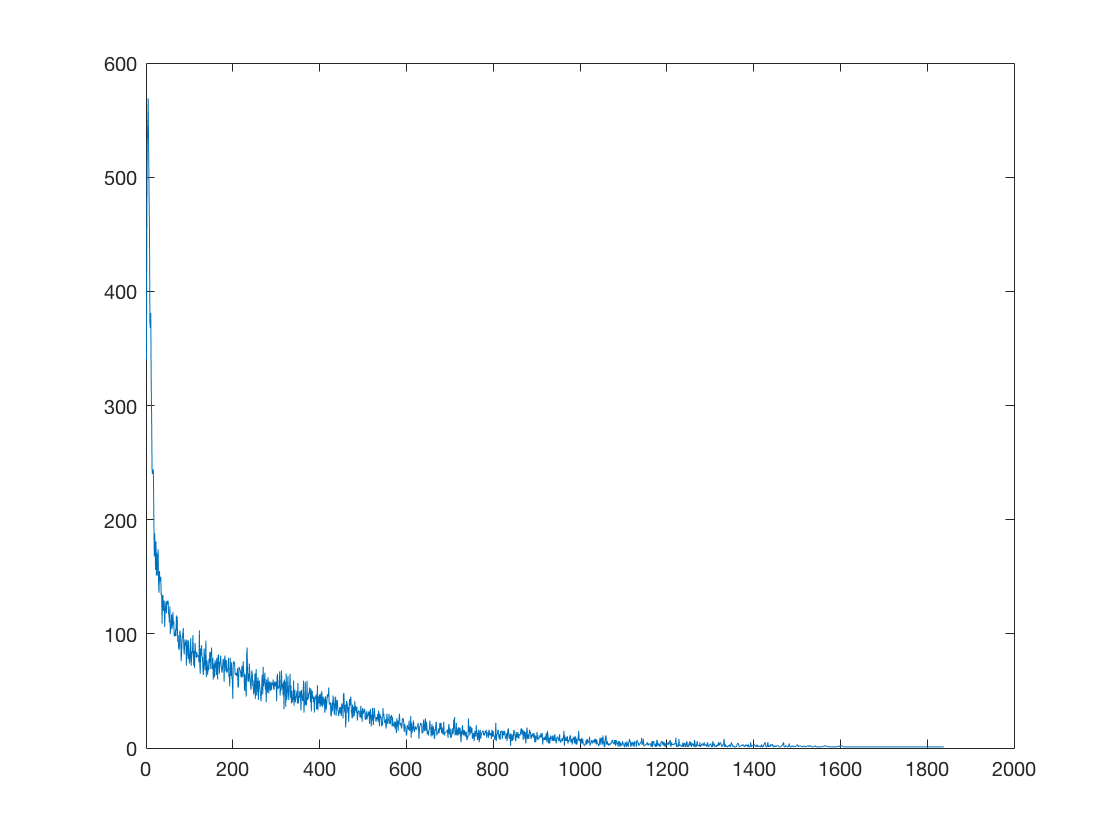
\includegraphics[width=80mm]{images/Count_vs_Days.png}
\caption{Bike Rental Frequency vs Count}
\label{countvsdays}
\end{figure}
\begin{center}
\begin{table}[ht!]
\centering
 \begin{tabular}{||c l l||} 
 \hline
 Value & Frequency & Class \\ [0.5ex] 
 \hline\hline
 1 & 1 - 40 & Can't see any bikes \\ 
 \hline
 2 & 40 - 200 & Very few bikes \\
 \hline
 3 & 200 - 400 & Less busy \\
 \hline
 4 & 400 - 600 & Normal \\
 \hline
 5 & 600 - 800 & Busy \\
 \hline
 6 & 800 - 1100 & Very Busy \\
 \hline
 7 & 1100 - 2000 & All bikes around \\ [1ex] 
 \hline
\end{tabular}
\caption{Classification of labels}
 \label{frequencyclasses}
\end{table}
\end{center}
\subsection{Train and Test data}
The data is split as training and test data based on the algorithm and the format of data the algorithm is expecting. For example, the input data for Bootstrap Aggregation, SVM and KNN will be in train and test data model, whereas the input for Classifier app is a single data file. The total number of data samples that are present are 46936 as the number of hours between January 2011 to June 2016 is 48192 and not all hours will the bikes be rented.\\
\indent For the models which require a split of data, we used random sampling and split the data as 40000 train samples and 6936 test samples which is equivalent to 85\% train data and 15\% test data.

\section{Related Work}
There is a significant amount of related work in Kaggle\textsuperscript{\cite{kaggle}} but for the subset of the data i.e., the data of the years 2011-2012 and for the different weather parameters. The models that are applied are in vast number and have no correlation between them. The models and kernels that are developed for this data doesn't address the reason behind applying that model and why the accuracy varies with the applied method and the parameters that drastically effect the models in detail. \\
\indent Our method of approach is different because the entire data set is constructed and the features are considered based on actual parameters that effect the bike rental frequency. As far as our knowledge is concerned, the best work done on this data so far is using Poisson's Regression\textsuperscript{\cite{relatedworkpoisson}}. Another paper\textsuperscript{\cite{relatedworkmultiple}} describes the models and the approaches that can be used in predicting the bike rental frequency but in a theoretical way. It compares the performance of Generalized Linear Models with Elastic Net Regularization (GLMNet), Generalized Boosted Models (GBM), Principal Component Regression (PCR), Support Vector Regression (SVR) and a kind of ensemble learning method called Stacking.

\section{Methods Used}
Considering all the models that are suitable for classification, we used a number of methods that can be trained for classification. The best algorithm is evaluated by getting the accuracy and implemented from scratch in Matlab to observe the importance of the parameters and if anyone of the default assumptions can be overridden for a better performance. The Classifier app\textsuperscript{\cite{classifier}} of Matlab and Math \& Stats model module in Matlab are used to calculate the accuracy of the predictions for all the above mentioned models. The methods varies from basic methods for classification to benchmark models. Following are some of such important methods:
\begin{itemize}
\item K-Nearest Neighbors (KNN) \textsuperscript{\cite{KNN}}
\item Support Vector Machines (SVM)\textsuperscript{\cite{libSVM}}
\item Support Vector Regression \textsuperscript{\cite{SVR}}
\item Discriminant (Linear and quadratic)\textsuperscript{\cite{lda}}
\item Classification Tree\textsuperscript{\cite{ctree}}
\item Ensemble Boosted Trees\textsuperscript{\cite{BoostedTrees}}
\item Ensemble Bagged Trees (Bootstrap Aggregation)\textsuperscript{\cite{bootstrapAggregation}}
\item Random Forest on Ensemble bagging trees\textsuperscript{\cite{randomForest}}
\item Rotation Forest\textsuperscript{\cite{rotationForest}} (New ensemble method)
\item Other models which are variants of the above mentioned models
\end{itemize}

\indent The algorithms that performed better than all other methods are \textit{Ensemble Bagged Trees (Bootstrap Aggregation)} and it's variation \textit{Random Forest on Ensemble bagging trees} with an average accuracy of 80\%.
\subsection{K-Nearest Neighbors (KNN)}
The K-Nearest neighbors\textsuperscript{\cite{KNN}} is best suited for classification mostly when dataset is too large, number of features is small and if the distance metric is good. KNN is considered inefficient in some cases as it consumes a lot of space sometimes reaching O(n\textsuperscript{d}). Variations of the KNN are verified and evaluated including Fine KNN, Medium KNN, Coarse KNN, Cosine KNN, Weighted KNN. 
\subsection{Support Vector Machines (SVM)}
Support Vector Machine models\textsuperscript{\cite{SVM}} for classification are best suited for binary classification. The SVM provided by the Math \& Statistical module in Matlab doesn't contain multi-class classification. Thus we used libsvm module\textsuperscript{\cite{libSVM}} which supports multi-class classification. In case of SVM models, the hyperparameters and regularizer have to be tuned to find the best match for any data set which is very challenging. The core functionality of SVM depends upon what kernel is being used and it is also challenging to pick the right kernel method. Since it also takes a lot of time to train the data and requires small amount of data samples and large amount of features to achieve better performance, SVM is almost unfit for this data set.
\subsection{Support Vector Regression}
Support Vector Machines\textsuperscript{\cite{SVR}} used for Regression are efficient only when the input data follows a pattern and thus establishes high correlation between the data samples. But SVR is highly insensitive to errors which makes this considerable, but the factors effecting the performance are the same as of SVM.
\subsection{Discriminant (Linear and quadratic)}
Linear and Quadratic discriminant analysis\textsuperscript{\cite{lda}} are best suitable only if the number of features are very large when compared to number of data samples. LDA requires an assumption of equal variance and co-variance matrices of the classes. The quadratic discriminant analysis comes somewhere in between the linear discriminant analysis and 1-NN (KNN with \textit{k}=1) and can be considered as a variant of LDA where heterogeneity of classes' co-variance matrices are accepted.
\subsection{Classification Tree}
The classification trees\textsuperscript{\cite{ctree}} or decision trees can be used to predict the class by selecting the most feature and evaluating the score for all the next features and choosing the next best optimal feature to make the split. The classification trees may overfit the data can also get struck in the local minima. Thus, ensemble methods are used which are described in the below sections.
\subsection{Ensemble Boosted Trees}
Boosting\textsuperscript{\cite{BoostedTrees}} is a method of decision also called as weak learning where the decision trees are also called as shallow trees since the level of trees is very less and the trees are often called as decision stumps. Boosting reduces bias of a large number of small models with low variance. However, Boosted trees are very sensitive to noise and outliers, and are very prone to overfitting.

\subsection{Ensemble Bagged Trees (Bootstrap Aggregation)}
Bootstrap Aggregation\textsuperscript{\cite{bootstrapAggregation}} or Bagging is a method of reducing the variance for high variance algorithms such as decision trees, Classification and Regression trees(CART). Bagging is a method where multiple models are created from the existing dataset by created sub-sample space. The models are trained and the average/ mode of all the predicted values is considered as the final predicted value. Bagging does not give importance to the individual underlying algorithms overfitting the training data. This is one of the best examples of Ensemble learning method. An ensemble learning method is defined as a learning model which collects and combines predictions from multiple machine learning models and combines the output to make more accurate predictions than the individual models. \\
\indent The individual decision trees are generally grown deep without pruning and will have high variance and low bias. The only parameters for Bagging decision trees are the number of sample and hence the number of trees. The number of trees are gradually increased run-by-run until accuracy became stable. The number of models can be very large and will not overfit the model.

\subsection{Random Forest on Ensemble bagging trees}
In Bagging decision trees, the predictions are highly correlated since the algorithms are greedy. Bagging works better if the predictions are uncorrelated or weakly correlated. To address this problem, Random Forest method\textsuperscript{\cite{randomForest}} is used. In a decision tree or CART, when choosing a split point, the learning algorithm looks at all options and choose one optimal split. The random forest model limits the number of choices to a random subset of features to search. Thus, an extra parameter (\textit{m}) is introduced here to specify how many features have to be searched at split point among all number of features(\textit{p}). Generally, the \textit{m} is defaulted to be square-root of \textit{p} in case of classification and \textit{p}/3 in case of regression. \\
\indent Once the data samples are selected in multiple sub-spaces, some samples will be left without taking into any of the sub sample space. These are called Out-Of-Bag samples (OOB) and are used to calculate the validation accuracy. An error function is calculated at each split point to validate the performance of the learning model. For classification, Gini score is the most used error function. Thus, random forests can be used to efficiently construct the learning model even for higher dimensional space and for large data samples. 

\subsection{Rotation Forest}
Rotation Forest\textsuperscript{\cite{rotationForest}} is a variation of random forest model where Principle Component Analysis(PCA)\textsuperscript{\cite{pca}} is applied for each individual sub-sample space of the random forest model. This is a new and experimental model where the accuracy is proven to be better than random forest and bagging models for some benchmark models. Thus, this is used for predicting the bike share frequency even though theoretically almost all the features/components are important in impacting the bike share frequency.

\section{Results}
Evaluating all the models (mentioned in Section V) in Matlab and also in Classifier App gave the individual accuracy of the models as in Table \ref{resultsAllAccuracies}.
\begin{center}
\begin{table}[ht!]
\centering
 \begin{tabular}{||l r||} 
 \hline
 Model & Accuracy (\%) \\ [0.5ex] 
 \hline\hline
Fine KNN & 50.2 \\
\hline
Medium KNN & 53.3 \\
\hline
Coarse KNN & 52.8 \\
\hline
Cosine KNN & 52.5 \\
\hline
Weighted KNN & 53.7 \\
\hline
Linear SVM & 48.3 \\
\hline 
Multi-class SVM & 63.0 \\
\hline
Support Vector Regression & 40.0\\
\hline 
Linear Discriminant & 47.0\\
\hline 
Quadratic Discriminant & 46.7\\
\hline
Simple Tree & 48.7\\
\hline 
Medium Tree & 55.4\\
\hline 
Complex Tree & 61.2\\
\hline 
Ensemble Subspace Displacement & 46.1\\
\hline
RUSBoosted Trees & 55.2\\
\hline 
Ensemble Boosted Trees & 57.5\\
\hline 
Ensemble subspace KNN & 60.8\\
\hline
Classification Trees (using fitctree) & 77.6\\
\hline 
Ensemble TreeBagger & 79.8 \\
\hline 
Ensemble Rotation Forest & 1 \\
\hline 
Ensemble Bagged Trees & 80.3\\[1ex] 
 \hline
\end{tabular}
\caption{Accuracies of all models used to predict the bike share frequency}
 \label{resultsAllAccuracies}
\end{table}
\end{center}

\subsection{K-Nearest Neighbors (KNN)}
The accuracy is highest at \textit{k} = 3.
\begin{figure}[ht!]
\centering
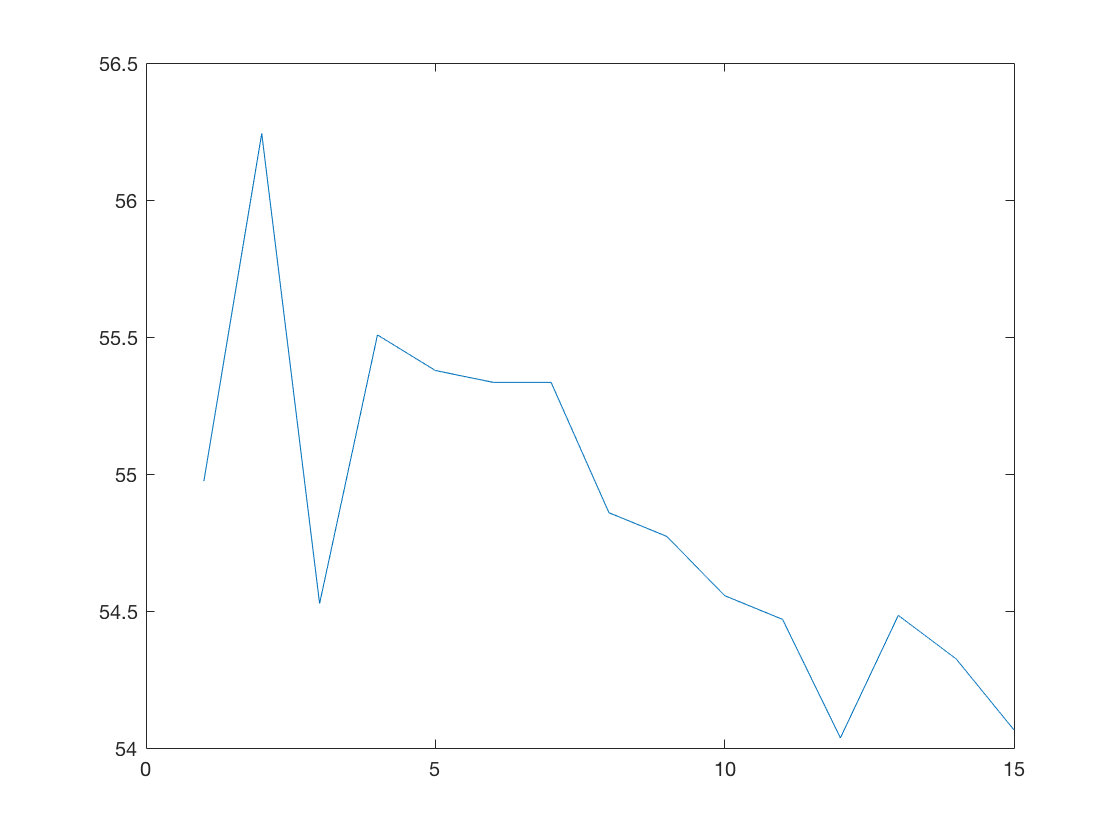
\includegraphics[width=80mm]{images/KNNClassifier.png}
\caption{KNN - K vs Accuracy}
\label{knnresults}
\end{figure}

\subsection{TreeBagger - Random Forest}
The TreeBagger is a class provided by the Math and Statistics module in Matlab to train the model using the ensemble bagging and also Random Forest method. The parameters that have to be changed here are the number of predictors that have to be changed for every split point (\textit{m}) and the number of decision trees that have to grown (\textit{N\textsubscript{t}}). Both the parameters are changed and the best optimal parameters are considered where accuracy is no longer improved.

\begin{figure}[ht!]
\centering
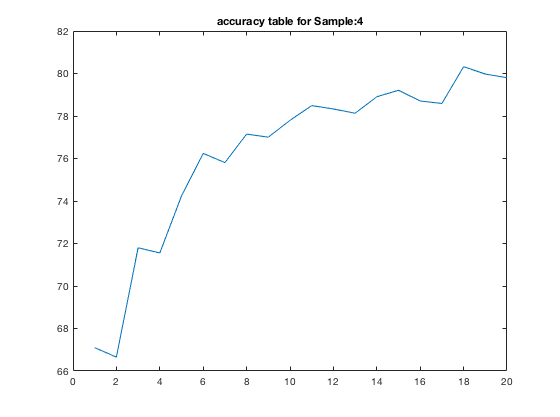
\includegraphics[width=80mm]{images/TBRF_num_predict_4.png}
\caption{TreeBagger Random Forest - Number of Trees vs Accuracy by fixing the \textit{m} = 4.}
\label{tbrfnumpred4}
\end{figure}

\begin{figure}[ht!]
\centering
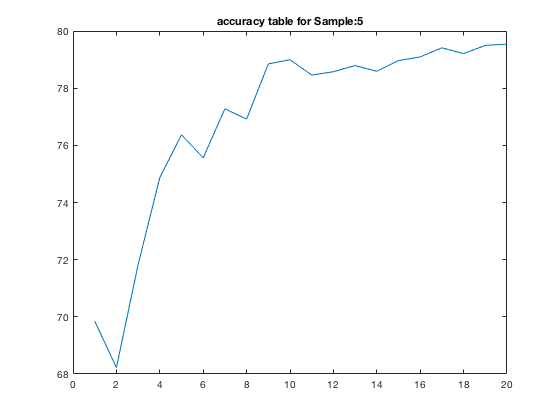
\includegraphics[width=80mm]{images/TBRF_num_predict_5.png}
\caption{TreeBagger Random Forest - Number of Trees vs Accuracy by fixing the \textit{m} = 5.}
\label{tbrfnumpred5}
\end{figure}

\begin{figure}[ht!]
\centering
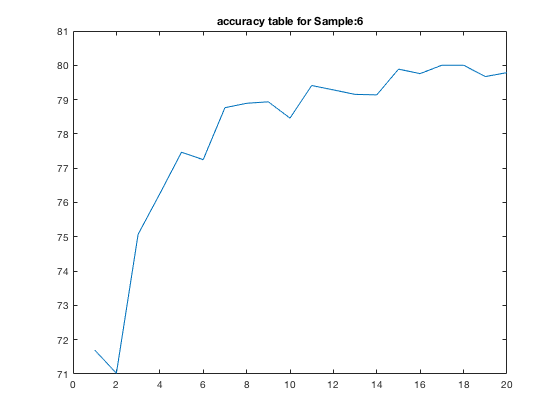
\includegraphics[width=80mm]{images/TBRF_num_predict_6.png}
\caption{TreeBagger Random Forest - Number of Trees vs Accuracy by fixing the \textit{m} = 6.}
\label{tbrfnumpred6}
\end{figure}

\begin{figure}[ht!]
\centering
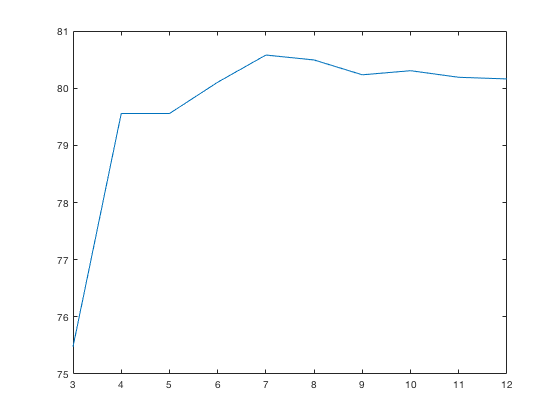
\includegraphics[width=80mm]{images/TBRF_numPredict_1_to_12.png}
\caption{TreeBagger Random Forest - Number of Predictors vs Accuracy by fixing the \textit{N\textsubscript{t}} = 10. The accuracy is optimal at \textit{m} = 7}
\label{tbrfnumpred7}
\end{figure}

\begin{figure}[ht!]
\centering
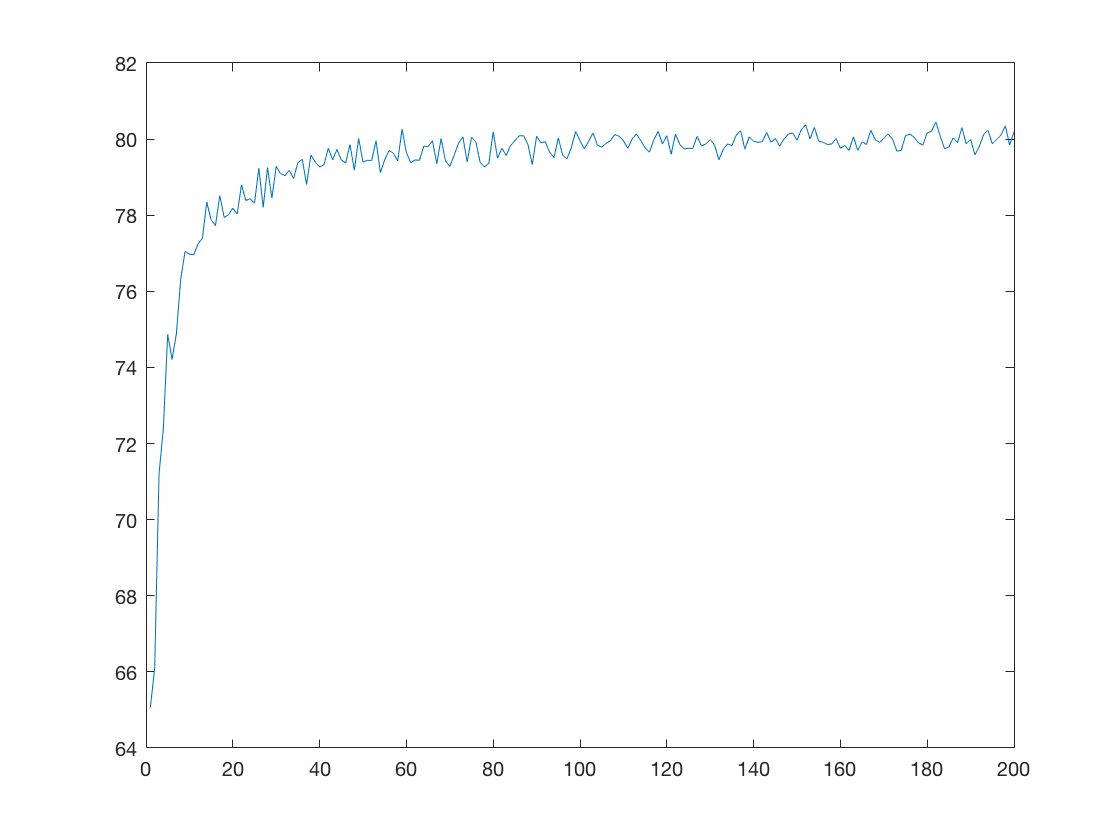
\includegraphics[width=80mm]{images/RandomForestPrediction200.png}
\caption{TreeBagger Random Forest - Number of Trees vs Accuracy by fixing the \textit{m} = 3 (default - square-root of \textit{p = 12}).}
\label{tbrfnumpred}
\end{figure}

\begin{figure}[ht!]
\centering
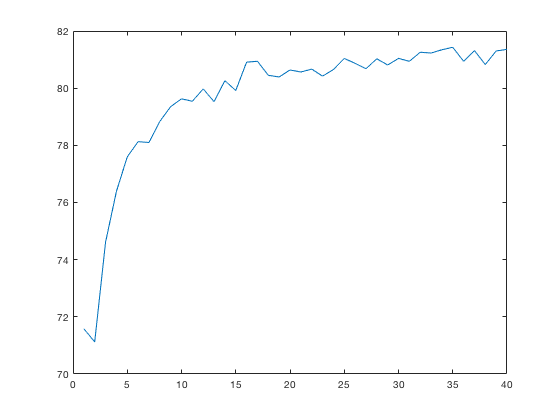
\includegraphics[width=80mm]{images/TBRF_NTrees_1_to_40.png}
\caption{TreeBagger Random Forest - Number of Decision trees vs Accuracy by fixing the \textit{m} = 7. The accuracy is optimal at \textit{N\textsubscript{t}} = 10}
\label{tbrfnumtrees}
\end{figure}

\subsection{Rotation Forest}
Rotation Forest is implemented on top of Random Forest implementation and the number of components for the PCA is the new parameter that is changed to calculate the accuracies. Figure \ref{rotationForestResults} shows the plot for the number of components selected and the accuracies of the learning models. For this, the size of sub sample size is fixed to be 20000 and the hyper parameter of the random forest model is set to 7.

\section{Conclusion}
We are fucked up as of now

\begin{thebibliography}{5}
    \bibitem{bsdataset} 
    Capital Bike Share Data-set\\
    \url{http://www.capitalbikeshare.com/system-data}
    \bibitem{weatherdata}
    Weather Data - ForecastIO - Washington DC\\
    \url{https://darksky.net/dev/docs/response}
    \bibitem{holidaydata}
    Holiday Schedule Data\\
    \url{http://dchr.dc.gov/page/holiday-schedules}
    \bibitem{kaggle}
    Kaggle\\
    \url{https://www.kaggle.com/c/bike-sharing-demand}
    \bibitem{relatedworkpoisson}
    Predictive bikeshare rebalancing\\
    \url{https://github.com/dssg/bikeshare}
    \bibitem{relatedworkmultiple}
    Jimmy Du, Rolland He, Zhivko Zhechev - \textit{Forecasting Bike Rental Demand}\\
    \url{http://cs229.stanford.edu/proj2014/Jimmy\%20Du,\%20Rolland\%20He,\%20Zhivko\%20Zhechev,\%20Forecasting\%20Bike\%20Rental\%20Demand.pdf}
    \bibitem{rotationForest}
    \textit{Rotation Forest: A New Classifier Ensemble Method} \\  
    \url{http://dl.acm.org/citation.cfm?id=1159358}
    
    \bibitem{randomForest}
    Leo Breiman and Adele Cutler - \textit{Random Forests}
    \url{https://www.stat.berkeley.edu/~breiman/RandomForests/cc_home.htm}
    
    \bibitem{bootstrapAggregation}
    \textit{Bagging and Random Forest Ensemble Algorithms for Machine Learning} \\
    \url{http://machinelearningmastery.com/bagging-and-random-forest-ensemble-algorithms-for-machine-learning/}
    
    \bibitem{KNN}
    \textit{K-Nearest Neighbors for Machine Learning} \\
    \url{http://machinelearningmastery.com/k-nearest-neighbors-for-machine-learning/}
    
    \bibitem{SVM}
    \textit{Support Vector Machines for Binary Classification}\\
    \url{https://www.mathworks.com/help/stats/support-vector-machines-for-binary-classification.html}
    
    \bibitem{libSVM}
    \textit{LIBSVM -- A Library for Support Vector Machines} \\
    \url{https://www.csie.ntu.edu.tw/~cjlin/libsvm/}
    
    \bibitem{SVR}
    \textit{Understanding Support Vector Machine Regression}\\
    \url{https://www.mathworks.com/help/stats/understanding-support-vector-machine-regression.html}
    
    \bibitem{lda}
    \textit{Linear discriminant analysis}\\
    \url{https://en.wikipedia.org/wiki/Linear_discriminant_analysis}
    
    \bibitem{ctree}
    Wei-Yin Loh - \textit{Classification and regression trees}\\
    \url{http://www.stat.wisc.edu/~loh/treeprogs/guide/wires11.pdf}
    
    \bibitem{BoostedTrees}
    Carlos Guestrin - \textit{Decision Trees Boosting}\\
    \url{http://www.cs.cmu.edu/~guestrin/Class/10701-S06/Slides/decisiontrees-boosting.pdf}
    
    \bibitem{BaggedTrees}
    Amit Srinet \& Dave Snyder - \textit{Bagging and Boosting}\\
    \url{https://www.cs.rit.edu/~rlaz/prec20092/slides/Bagging_and_Boosting.pdf}
    
    \bibitem{bikesharewiki}
    \textit{Bicycle-sharing system}\\
    \url{https://en.wikipedia.org/wiki/Bicycle-sharing_system}
    
    \bibitem{capitalbikeshare}
    \textit{Capital Bike Share}\\
    \url{http://www.capitalbikeshare.com/}
    
    \bibitem{classifier}
    \textit{Classification Learner - Matlab App}\\
    \url{https://www.mathworks.com/help/stats/classificationlearner-app.html}
    
    \bibitem{pca}
    \textit{Principal Component Analysis}\\
    \url{https://en.wikipedia.org/wiki/Principal_component_analysis}
    
    \bibitem{}
    \textit{}\\
    \url{}
    
    \bibitem{}
    \textit{}\\
    \url{}
    
    \bibitem{}
    \textit{}\\
    \url{}
    
    \bibitem{}
    \textit{}\\
    \url{}
    
    \bibitem{}
    \textit{}\\
    \url{}
    
    
    
    
    
    
\end{thebibliography}
\end{document}